\PassOptionsToPackage{dvipsnames,svgnames,table}{xcolor}
\documentclass[11pt]{article}
\usepackage[a4paper,margin=22mm]{geometry}
\usepackage[no-math]{fontspec}
\setmainfont{DejaVu Serif}
\usepackage{amsmath,amssymb,amsthm,mathtools,graphicx,xcolor,hyperref,xurl,xspace,ifthen,enumerate}
\usepackage[shortlabels]{enumitem}
\setlength{\emergencystretch}{4em}
\AtBeginDocument{\special{pdf:mapline pzdr Dingbats <uzdr.pfb}}
\SetMathAlphabet{\mathbf}{normal}{OT1}{cmr}{bx}{n}
\SetMathAlphabet{\mathbf}{bold}{OT1}{cmr}{bx}{n}
\newtheorem{theo}{Theorem}[section]
\newtheorem{lemm}[theo]{Lemma}
\newtheorem{thm}[theo]{Theorem}
\newtheorem{proposition}[theo]{Proposition}
\newtheorem{corollary}[theo]{Corollary}
\newtheorem{definition}[theo]{Definition}
\newtheorem{theorem}[theo]{Theorem}
\newtheorem*{remas*}{Remarks}
\newtheorem{remas}[theo]{Remarks}
\newtheorem*{exam*}{Example}
\newtheorem{ques}[theo]{Question}
\providecommand{\og}{«\nobreakspace}
\providecommand{\fg}{\nobreakspace»}
\newtheorem{lem}[theo]{Lemma}
\newtheorem{lemma}[theo]{Lemma}
\newtheorem{prop}[theo]{Proposition}
\newtheorem{coro}[theo]{Corollary}
\newtheorem{corol}[theo]{Corollary}
\newtheorem*{conj*}{Conjecture}
\newtheorem{conj}[theo]{Conjecture}
\newtheorem{conjecture}[theo]{Conjecture}
\newtheorem{Proposition}[theo]{Proposition}
\newtheorem{theoreme}[theo]{Theorem}
\theoremstyle{definition}
\newtheorem{defi}[theo]{Definition}
\newtheorem{exam}[theo]{Example}
\newtheorem{exem}[theo]{Example}
\newtheorem{remark}[theo]{Remark}
\newtheorem{example}[theo]{Example}
\newtheorem{exams}[theo]{Examples}
\newtheorem{rema}[theo]{Remark}
\newtheorem{nota}[theo]{Notation}
\newtheorem{notation}[theo]{Notation}
\newtheorem*{notas}{Notations}
\newtheorem{result}[theo]{Result}
\newtheorem{question}[theo]{Question}
\newtheorem{prob}[theo]{Problem}
\newtheorem*{rema*}{Remark}
\newtheorem*{defi*}{Definition}
\newtheorem*{theo*}{Theorem}
\newtheorem*{lemm*}{Lemma}
\newtheorem*{prop*}{Proposition}
\newcommand{\enoncename}{}
\newtheorem{corpusenonce}[theo]{\enoncename}
\newenvironment{enonce}[2][]{\renewcommand{\enoncename}{#2}\begin{corpusenonce}}{\end{corpusenonce}}
\newenvironment{enonce*}[2][]{\par\medskip\noindent\textbf{#2.}\itshape}{\par\medskip}
\newenvironment{proofc}[1][\proofname]{\begin{proof}[#1]}{\end{proof}}
\newcommand{\Mc}{\mathcal{M}}
\newcommand{\pointir}{.\ ---\ }
\newcommand{\equalenv}[2]{\expandafter\let\csname#1\expandafter\endcsname\csname#2\endcsname\expandafter\let\csname end#1\expandafter\endcsname\csname end#2\endcsname}
\providecommand{\diagbox}[3][]{\begin{tikzpicture}[x=1em,y=1em,baseline=(current bounding box.center)]\useasboundingbox(0,0) rectangle(3,1.4);\draw(0,1.4)--(3,0);\node at(.5,.3){#2};\node at(2.5,1.1){#3};\end{tikzpicture}}
\providecommand{\eg}{e.g.\ }
\providecommand{\ie}{i.e.\ }
\providecommand{\cf}{cf.\ }
\providecommand{\longthanks}[1]{\par\smallskip\noindent #1\par\smallskip}
\providecommand{\qbinom}[2]{\genfrac{[}{]}{0pt}{}{#1}{#2}}

\providecommand{\mathof}[1]{\mathrm{#1}}

\numberwithin{equation}{section}


\def\endappendix{}


\usepackage{xcolor}

\definecolor{darkblue}{rgb}{0.0,0.0,0.7}

\usepackage{tikz}
\usetikzlibrary{trees, decorations, decorations.markings, shapes, arrows, matrix, calc, fit, intersections, patterns, angles, automata, positioning}

\newcommand{\N}{\mathbb{N}}
\newcommand{\Z}{\mathbb{Z}}
\newcommand{\Q}{\mathbb{Q}}
\newcommand{\R}{\mathbb{R}}
\newcommand{\C}{\mathbb{C}}
\newcommand{\fS}{\mathfrak{S}}

\newcommand{\set}[2]{\left\{ #1 \;\middle|\; #2 \right\}}
\newcommand{\bigset}[2]{\big\{ #1 \;\big|\; #2 \big\}}
\newcommand{\ssm}{\smallsetminus}
\newcommand{\dotprod}[2]{\left\langle \, #1 \; \middle| \; #2 \, \right\rangle}
\newcommand{\symdif}{\,\triangle\,}
\newcommand{\one}{\b{1}}
\newcommand{\eqdef}{\mbox{\,\raisebox{0.2ex}{\scriptsize\ensuremath{\mathrm:}}\ensuremath{=}\,}}
\newcommand{\defeq}{\mbox{~\ensuremath{=}\raisebox{0.2ex}{\scriptsize\ensuremath{\mathrm:}} }}
\newcommand{\defn}[1]{\textsl{\color{darkblue} #1}}
\newcommand{\apriori}{\textit{a priori}}
\newcommand{\viceversa}{\textit{vice versa}}
\newcommand{\versus}{\textit{vs.}~}
\newcommand{\aka}{\textit{a.k.a.}~}
\newcommand{\perse}{\textit{per se}}
\DeclareMathOperator{\inv}{inv}
\DeclareMathOperator{\ninv}{ninv}
\DeclareMathOperator{\moveU}{moveU}
\DeclareMathOperator{\moveD}{moveD}

\newcommand{\automatonA}{\mathbb{A}}
\newcommand{\automatonP}{\mathbb{P}}
\newcommand{\automatonU}{\mathbb{U}}
\newcommand{\automatonD}{\mathbb{D}}
\newcommand{\length}{\ell}
\newcommand{\generatingTree}{\mathcal{T}}
\newcommand{\lexmin}{\mathcal{R}}

\begin{document}
\section*{\raggedright 1101: Disjoint up-down permutree avoidance is equivalent to simultaneous reduced-word automaton acceptance}
\noindent\textbf{Author:} Pilaud, Vincent; Pons, Vivane; Tamayo Jimenez, Daniel\par\noindent\textbf{Source:} Permutree sorting. Algebraic Combinatorics 6 (2023), publisher version, DOI 10.5802/alco.249. \url{https://alco.centre-mersenne.org/articles/10.5802/alco.249/}
\par\noindent\textbf{License:} CC BY 4.0, \url{https://creativecommons.org/licenses/by/4.0/}. The original publisher PDF cover has the explicit license notice. See the saved source/license records.
\par\noindent\textbf{Editorial material note (not author text):} The selected problem is exact original Theorem1.2 for disjoint U,D subsets of\{2,...,n-1\}: existence of one reduced word simultaneously accepted by all specified automata is equivalent to all authored jki/kij avoidance conditions. Complete source Sections1--2, required Section3.1 and Section4.1 retain recursive/complete automaton definitions, every single-label transition/avoidance lemma and proof, refined terminal-state/noninversion proposition with full induction, and the full common-word construction969--990. The new obligation synchronizes distinct independently accepted automata; an unrestricted overlap U intersection D is not claimed. Later sorting algorithms, generating trees and c-sorting comparisons are unselected and only their exact original printed locators remain. Every automaton figure is fully editable author TikZ, all general mathematical text and proof native TeX. Genuinely unused hvfloat/cancel/algorithm2e/tkz-graph imports are omitted after complete active-control/environment inventory; no package emulation, math repair or generated proof. All proof text and formulas below are editable author TeX. Mathematical wording, language and proof order are retained. Only the article class, title matter and bibliography presentation are adapted for independent compilation; no proof has been generated or repaired.
\par\noindent\textbf{Editorial difficulty:} H2: The proof constructs a common sorting word for a permutation individually accepted by multiple interacting automata, controlling invariant noninversion sets and forced adjacent swaps. A maximal forbidden-label argument lets the author synchronize all up/down constraints without creating new prohibited patterns, beyond a single stack-sortability criterion.
\medskip\hrule\medskip
\noindent\textbf{Author statement, complete proof and local supporting text follow in source order.}
\section{Introduction}

The weak order is a classical lattice on the symmetric group where permutations are ordered by inclusion of inversion sets.
Generalizing the classical Tamari lattice~\cite{Tamari}, N.~Reading studied the lattice quotients of the weak order~\cite{Reading-latticeCongruences}, in particular the Cambrian lattices~\cite{Reading-cambrianLattices,Reading-coxeterSortable}.
Generalizing and interpolating between the weak order, the Cambrian lattices and the boolean lattice, we introduced permutree lattices in~\cite{PilaudPons-permutrees} based on the combinatorics of certain trees called permutrees.
These permutree lattices have strong combinatorial, geometric and algebraic properties distinguishing them among all lattice quotients of the weak order: for instance, they are the only lattice quotients of the weak order which can be realized as removahedra~\cite{AlbertinPilaudRitter-Removahedra} (\ie polytopes obtained by removing inequalities in the facet description of the classical permutahedra, like the classical associahedra of~\cite{Loday,HohlwegLange}), and they define combinatorial Hopf algebras~\cite{PilaudPons-permutrees} analoguous to the Hopf algebras of C.~Malvenuto and C.~Reutenauer on permutations~\cite{MalvenutoReutenauer} and of J.-L.~Loday and M.~Ronco on binary trees~\cite{LodayRonco}.



Unlike Cambrian lattices which are well-understood for arbitrary finite Coxeter groups~\cite{Reading-cambrianLattices,Reading-coxeterSortable} with their connections to finite type cluster algebras~\cite{FominZelevinsky-ClusterAlgebrasI,FominZelevinsky-ClusterAlgebrasII}, permutree lattices lack a combinatorial description beyond the symmetric group.
To tackle this problem, this paper still focusses on type~$A$ permutree lattices but from the lens of reduced words for permutations (\ie products of simple transpositions of minimal length).
This approach not covered in \cite{PilaudPons-permutrees} is more suitable to generalizations to finite Coxeter groups.

The goal of this paper is to identify reduced words which correspond to the minimal permutations of their permutree congruence classes.
These permutations are generalizations of the \defn{stack-sortable} permutations introduced by D.~Knuth in his textbook~\cite[Sect.~2.2.1]{Knuth-TAOCP1}, which are characterized by the following equivalent conditions for a permutation~$\pi \in \fS_n$:
\begin{enumerate}[(i)]
\item \label{condition:stackSorting}
$\pi$ is sent to the identity by the stack sorting operator~$S$ defined inductively by~$S(\tau n \rho) \eqdef S(\tau) S(\rho) n$.
\item \label{condition:patternStack}
$\pi$ avoids the pattern $231$ (\ie there is no~$p < q < r$ such that~$\pi_r < \pi_p < \pi_q$).
\item \label{condition:minimalLinearExtentionBinaryTree}
$\pi$ is minimal among all linear extensions of a binary tree on $n$ nodes (seen as a poset, where the nodes are labeled in inorder and the edges are oriented towards the leaves).
\item \label{condition:alignedStack}
For $i < j < k$, the inversion set~$\inv(\pi) \eqdef \set{(\pi_p, \pi_q)}{p < q \text{ and } \pi_p > \pi_q}$ of~$\pi$ contains the inversion $(k,j)$ as soon as it contains the inversion~$(k,i)$.
\item \label{condition:sortableStack}
$\pi$ admits a reduced word of the form~$\pi = c_{I_1} \cdots c_{I_p}$ with nested subsets ${I_1 \supseteq \dots \supseteq I_p}$, where~$c_{\{i_1 < \dots < i_j\}} \eqdef s_{i_j} \cdots s_{i_1}$ is a product of the simple transpositions~$s_i \eqdef (i \;\; i+1)$.
\end{enumerate}
It follows from~\ref{condition:minimalLinearExtentionBinaryTree} that these permutations are counted by the Catalan number~$C_n \eqdef \frac{1}{n+1} \binom{2n}{n}$.

In~\cite{Reading-latticeCongruences, Reading-cambrianLattices, Reading-coxeterSortable}, N.~Reading defined natural counterparts to conditions~\ref{condition:minimalLinearExtentionBinaryTree}, \ref{condition:alignedStack}, and~\ref{condition:sortableStack} above, parametrized by the choice of a Coxeter element~$c$ in a finite Coxeter group~$W$: the minimality in $c$-Cambrian classes, the $c$-alignment, and the $c$-sortability.
(We skip the general definitions of these conditions here as we stick with the combinatorics of the symmetric group.)
In the situation of the symmetric group~$\fS_n$, we can think of a Coxeter element on~$\fS_n$ as an orientation of an $(n-1)$-path, or equivalently as a partition of~$\{2, \dots, n-1\}$ into two subsets~$U$ and~$D$.
The Cambrian analogues of the conditions~\ref{condition:patternStack}, \ref{condition:minimalLinearExtentionBinaryTree}, \ref{condition:alignedStack} and~\ref{condition:sortableStack} above are the following equivalent conditions for a permutation~$\pi \in \fS_n$:
\begin{enumerate}[(i')]
\addtocounter{enumi}{1}
\item \label{condition:patternCambrian}
For~$i < j < k$, the permutation~$\pi$ does not contain the subword $jki$ if~$j \in U$ and~$kij$ if~$j \in D$.
\item \label{condition:minimalLinearExtentionCambrian}
$\pi$ is minimal among all linear extensions of a $c$-Cambrian tree on $n$ nodes. A $c$-Cambrian tree is an oriented tree on~$[n]$ where node~$j$ has one parent if~$j \notin U$ and two parents if~$j \in U$, and one child if~$j \notin D$ and two children if~$j \in D$, with an additional local condition at each node similar to the binary search tree condition~\cite{ChatelPilaud}.
\item \label{condition:alignedCambrian}
For~$i < j < k$, if~$\inv(\pi)$ contains~$(k,i)$, then it also contains $(k,j)$ if~$j \in U$ and $(j,i)$ if $j \in D$.
\item \label{condition:sortableCambrian}
$\pi$ admits a reduced word of the form~$\pi = c_{I_1} \cdots c_{I_p}$ with nested subsets ${I_1 \supseteq \dots \supseteq I_p}$, where~$c_I \eqdef c_{i_1} \cdots c_{i_{|I|}}$ denotes the subword of~$c \eqdef c_1 \cdots c_{n-1}$ indexed by~$I \eqdef \{i_1 < \dots < i_j\}$.
\end{enumerate}
It turns out that for any Coxeter element~$c$, the permutations satisfying these conditions are still counted by the Catalan number~$C_n$.

The generalization to permutrees consists of taking two subsets~$U$ and~$D$ of~$\{2, \dots, n-1\}$ that are not anymore required to form a partition of~$\{2, \dots, n-1\}$ (they may intersect and may not cover all the set).
It was proved in~\cite{PilaudPons-permutrees, ChatelPilaudPons} that the conditions~\ref{condition:patternCambrian}, \ref{condition:minimalLinearExtentionCambrian}, and~\ref{condition:alignedCambrian} are still equivalent for a permutation~$\pi \in \fS_n$.
We call a permutation \defn{$(U,D)$-permutree minimal} when it satisfies these conditions, \ie when it is minimal (minimal number of inversions) in its $(U,D)$-permutree class.
The number of $(U,D)$-permutree minimal permutations is called $(U,D)$-factorial-Catalan number and admits recursive formulae interpolating between the formulae for the factorial and for the Catalan number.

The objective of this paper is to discuss characterizations of permutree minimal permutations in terms of their reduced words.
In other words, we aim at a condition playing the role of condition~\ref{condition:sortableCambrian} and equivalent to conditions~\ref{condition:patternCambrian}, \ref{condition:minimalLinearExtentionCambrian}, and~\ref{condition:alignedCambrian} for arbitrary subsets~$U$ and~$D$ of~$\{2, \dots, n-1\}$.
We believe that understanding this characterization in type~$A$ could lead to a general characterization for all finite Coxeter groups since the condition~\ref{condition:sortableCambrian} generalizes to all types for Cambrian lattices.

We first focus on the case where~$U = \varnothing$ and~$D = \{j\}$ for some~${j \in \{2, \dots, n-1\}}$, or the opposite.
To characterize the permutree minimal permutations in terms of their reduced words in that situation, we use two automata~$\automatonU(j)$ and $\automatonD(j)$ defined inductively as shown in Figure~\ref{fig:automataRecursive}.
The induction stops at~$\automatonU(n)$ and~$\automatonD(1)$, which are defined by deleting the transitions~$s_n$ and~$s_0$ respectively in Figure~\ref{fig:automataRecursive}.
Figure~\ref{fig:automataComplete} presents the complete automaton $\automatonU(j)$ after all recursion is done, and Figure~3 shows the automata~$\automatonU(2)$, $\automatonD(2)$, $\automatonU(3)$, and~$\automatonD(3)$.
In all these pictures the initial state is marked with ``start'', the accepting states are doubly circled, all transitions are labeled with simple transpositions~$s_i$ for~$i \in [n-1]$, and all missing transitions are loops (we assume the reader familiar with basic automata theory, see for instance~\cite{HopcroftUllman}).
Our main tool is the following statement, proved in Section~\ref{sec:proofPatternAvoidance}.

\begin{theorem}\label{thm:patternAvoidance}
Fix $j \in \{2, \dots, n-1\}$.
The following conditions are equivalent for~${\pi \in \fS_n}$:
\begin{itemize}
	\item $\pi$ admits a reduced word accepted by the automaton~$\automatonU(j)$ (resp.~$\automatonD(j)$),
	\item $\pi$ contains no subword $jki$ (resp.~$kij$) with~$i < j < k$.
\end{itemize}
\end{theorem}

Let us warn the reader on the fact that~$j$ is fixed in Theorem~\ref{thm:patternAvoidance}, while $i$ and~$k$ are arbitrary such that~$1 \le i < j < k \le n$.
A priori, we should try all possible reduced words of~$\pi$ to decide if one is accepted by the automaton~$\automatonU(j)$ (resp.~$\automatonD(j)$).
However, we can show that if~$\pi$ contains no subword $jki$ (resp.~$kij$) with~${i < j < k}$ and has a descent~$s_\ell$ distinct from~$s_{j-1}$ (resp.~$s_j$), then it has a reduced word starting with~$s_\ell$ and accepted by the automaton~$\automatonU(j)$ (resp.~$\automatonD(j)$).
In other words, there is no loss of generality in starting constructing a reduced word for~$\pi$ as long as we stay in the states of the top row of~$\automatonU(j)$ (resp.~$\automatonD(j)$).
This yields a simple algorithm to construct a reduced word accepted by~$\automatonU(j)$ (resp.~$\automatonD(j)$).
It also yields natural tree structures on the permutations characterized by Theorem~\ref{thm:patternAvoidance}, which can be glanced upon in Figure~3.
These algorithmic and combinatorial consequences of Theorem~\ref{thm:patternAvoidance} are explored in Section~\ref{sec:algorithmicCombinatorialConsequences}.
Most results of Sections~\ref{sec:proofPatternAvoidance} and~\ref{sec:algorithmicCombinatorialConsequences} are stated with respect to both automata~$\automatonU(j)$ and $\automatonD(j)$ but proved only for $\automatonU(j)$ as all proofs for~$\automatonD(j)$~are~symmetric.

\begin{figure}
	\centerline{
		$\automatonU(j) \eqdef$
		\begin{tikzpicture}[shorten >=1pt, node distance=2cm, on grid, auto, baseline=-1.5cm]
			\node[state,initial,accepting,minimum size=0.5cm] (q_0) {}; 
			\node[state,accepting,minimum size=0.5cm] (q_1) [below= 1.5cm of q_0] {}; 
			\node[state,minimum size=0.5cm] (q_2) [below= 1.5cm of q_1] {}; 
			\node (q_3) [right= 2.5cm of q_0] {$\automatonU(j+1)$};
			\path[->] 
				(q_0) edge node [swap] {$s_{j-1}$} (q_1)
					  edge node {$s_j$} (q_3)
				(q_1) edge node [swap] {$s_j$} (q_2);
		\end{tikzpicture}
		\quad \,
		$\automatonD(j) \eqdef$
		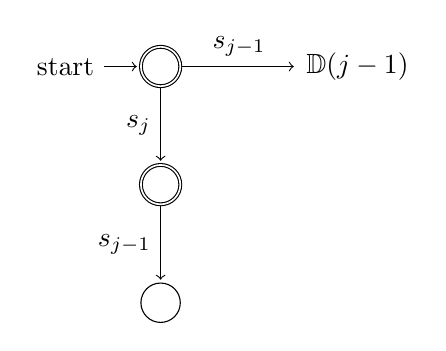
\begin{tikzpicture}[shorten >=1pt, node distance=2cm, on grid, auto, baseline=-1.5cm] 
			\node[state,initial,accepting,minimum size=0.5cm] (q_0) {}; 
			\node[state,accepting,minimum size=0.5cm] (q_1) [below= 1.5cm of q_0] {}; 
			\node[state,minimum size=0.5cm] (q_2) [below= 1.5cm of q_1] {}; 
			\node (q_3) [right= 2.5 cm of q_0] {$\automatonD(j-1)$};
			\path[->] 
				(q_0) edge node [swap] {$s_{j}$} (q_1)
					  edge node {$s_{j-1}$} (q_3)
				(q_1) edge node [swap] {$s_{j-1}$} (q_2);
		\end{tikzpicture}
	}
	\caption{The automata $\automatonU(j)$ (left) and $\automatonD(j)$ (right) defined recursively.}
	\label{fig:automataRecursive}
\end{figure}

\begin{figure}
	\centerline{
		\scalebox{0.9}{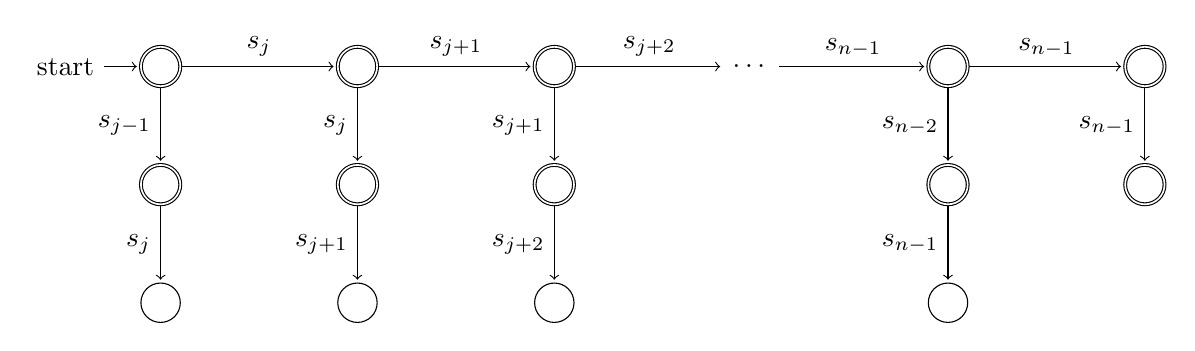
\begin{tikzpicture}[shorten >=1pt, node distance=2cm, on grid, auto]
			\node[state,initial,accepting,minimum size=0.5cm] (hj-1)   {}; 
			\node[state,accepting,minimum size=0.5cm] (ij-1) [below= 1.5cm of hj-1] {}; 
			\node[state,minimum size=0.5cm] (dj-1) [below= 1.5cm of ij-1] {}; 
			\node[state,accepting,minimum size=0.5cm] (hj) [right= 2.5cm of hj-1] {};
			\node[state,accepting,minimum size=0.5cm] (ij) [below= 1.5cm of hj] {}; 
			\node[state,minimum size=0.5cm] (dj) [below= 1.5cm of ij] {}; 
			\node[state,accepting,minimum size=0.5cm] (hj+1) [right= 2.5cm of hj] {};
			\node[state,accepting,minimum size=0.5cm] (ij+1) [below= 1.5cm of hj+1] {}; 
			\node[state,minimum size=0.5cm] (dj+1) [below= 1.5cm of ij+1] {};	  
			\node (void) [right= 2.5cm of hj+1] {\dots};
			\node[state,accepting,minimum size=0.5cm] (hn-2) [right= 2.5cm of void] {};
			\node[state,accepting,minimum size=0.5cm] (in-2) [below= 1.5cm of hn-2] {}; 
			\node[state,minimum size=0.5cm] (dn-2) [below= 1.5cm of in-2] {}; 
			\node[state,accepting,minimum size=0.5cm] (hn-1) [right= 2.5cm of hn-2] {}; 
			\node[state,accepting,minimum size=0.5cm] (in-1) [below= 1.5cm of hn-1] {}; 
			\path[->] 
				(hj-1) edge node [swap] {$s_{j-1}$} (ij-1)
					   edge node {$s_j$} (hj)
				(ij-1) edge node [swap] {$s_j$} (dj-1)
				(hj) edge node [swap] {$s_{j}$} (ij)
					 edge node {$s_{j+1}$} (hj+1)
				(ij) edge node [swap] {$s_{j+1}$} (dj)			
				(hj+1) edge node [swap] {$s_{j+1}$} (ij+1)
					   edge  node {$s_{j+2}$} (void)
				(ij+1) edge  node [swap] {$s_{j+2}$} (dj+1)			  
				(void) edge node {$s_{n-1}$} (hn-2)
				(hn-2) edge node [swap] {$s_{n-2}$} (in-2)
					   edge node {$s_{n-1}$} (hn-1)
				(in-2) edge node [swap] {$s_{n-1}$} (dn-2)
				(hn-1) edge node [swap] {$s_{n-1}$} (in-1);
		\end{tikzpicture}}
		}
	\caption{The complete automaton~$\automatonU(j)$.}
	\label{fig:automataComplete}
\end{figure}

Consider now arbitrary subsets~$U$ and~$D$ of~$\{2, \dots, n-1\}$.
It follows from Theorem~\ref{thm:patternAvoidance} that a permutation is minimal in its $(U,D)$-permutree class if and only if it admits a reduced word accepted by~$\automatonU(j)$ for each~$j \in U$ and by~$\automatonD(j)$ for each~$j \in D$.
In general, the reduced words accepted by the automata~$\automatonU(j)$ for each~$j \in U$ and by~$\automatonD(j)$ for each~$j \in D$ are distinct.
We prove however in Section~\ref{sec:intersectionsAutomata} that there is a reduced word simultaneously accepted by all these automata when~$U$ and~$D$ are~disjoint.

\begin{theorem}\label{thm:permutreeMinimal}
Consider two disjoint subsets~$U$ and~$D$ of~$\{2, \dots, n-1\}$.
The following conditions are equivalent for~$\pi \in \fS_n$:
\begin{itemize}
	\item $\pi$ admits a reduced word accepted by all automata~$\automatonU(j)$ for~$j \in U$ and~$\automatonD(j)$ for~${j \in D}$,
	\item $\pi$ contains no subword $jki$ if~$j \in U$ and~$kij$ if~$j \in D$ for any~$i < j < k$.
\end{itemize}
\end{theorem}

Theorem~\ref{thm:permutreeMinimal} implies that given any permutation~$\pi$ avoiding $jki$ if~$j \in U$ and~$kij$ if~$j \in D$, we can sort~$\pi$ while preserving these avoiding conditions.
The resulting sorting procedures, that we call \defn{$(U,D)$-permutree sorting}, are discussed in~Section~4.4.
For instance, stack sorting is a $(\{2, \dots, n-1\}, \varnothing)$-permutree sorting.

Finally, in the particular situation when the subsets~$U$ and~$D$ form a partition of~$\{2, \dots, n-1\}$, we actually show that the reduced word simultaneously accepted by the automata $\automatonU(j)$ for~${j \in U}$ and~$\automatonD(j)$ for~$j \in D$ is the $c$-sorting word of~$\pi$ as defined in~\cite{Reading-coxeterSortable}.
This yields in particular an alternative proof that condition~\ref{condition:sortableCambrian} characterizes the Cambrian minimal permutations.
This new perspective on $c$-sortability is explored in Section~5.

\section{Automata for reduced words}\label{sec:proofPatternAvoidance}

\subsection{Reduced words, automata, and subword avoidance}

We start with properly fixing the few notations needed in this paper.
We consider the \defn{symmetric group}~$\fS_n$ of permutations of the set~$[n] \eqdef \{1,\dots,n\}$.
It is generated by the \defn{simple transpositions}~$s_i \eqdef (i \;\; i+1)$ for $i \in [n-1]$ which are involutions~$s_i^2 = id$ and satisfy the commutation relations $s_i \cdot s_j =s_j \cdot s_i$ if $|i-j|>1$ and the braid relations~$s_i \cdot s_{i+1} \cdot s_i = s_{i+1} \cdot s_i \cdot s_{i+1}$.
Note that we multiply permutations as usual, so that the left multiplication by~$s_i$ exchanges the entries with values~$i$ and~$i+1$, while the right multiplication by~$s_i$ exchanges the entries at positions~$i$ and~$i+1$.
Each permutation~$\pi$ decomposes into products of transpositions of the form~$\pi = s_{i_1} \cdots s_{i_k}$ with~$i_1, \dots, i_k \in [n-1]$.
The minimal number of transpositions in such a decomposition is the \defn{length}~$\ell(\pi)$ of~$\pi$ and the decompositions of length~$\ell(\pi)$ are \mbox{the \defn{reduced words} for~$\pi$}.

Consider now the automata $\automatonU(j)$ and $\automatonD(j)$ described in the introduction, see Figures~\ref{fig:automataRecursive},~\ref{fig:automataComplete}, and~3.
We call a state \defn{healthy}, \defn{ill}, or \defn{dead} depending on whether it belongs to the top, middle, or bottom row of the automata.
Each state has $n-1$ possible transitions, one for each $s_i$ for~$i \in [n-1]$, but we only explicitly indicate the ones between different states.
The automata $\automatonU(j)$ and $\automatonD(j)$ take as entry a reduced word~$s_{i_1} \cdots s_{i_\ell}$ for a permutation of~$\fS_n$ and read it from left to right.
We start at the initial state (marked with ``start''), and at step~$t$ we follow the transition marked by the letter~$s_{i_t}$ if any, or stay in the current state otherwise.
After~$\ell$ steps, the reduced word~$s_{i_1} \cdots s_{i_\ell}$ is declared accepted if the current state is accepting (doubly circled, healthy or ill states), and rejected otherwise (dead states).

For a fixed~$j \in \{2, \dots, n-1\}$, we say that a permutation~$\pi$ \defn{avoids} $jki$ (resp.~$kij$) if for any~$i < j < k$, the word~$jki$ (resp.~$kij$) does not appear as a subword of the one-line notation of~$\pi$, or said differently if there are no positions~$p < q < r$ such that~$\pi(r) < \pi(p) = j < \pi(q)$ (resp.~$\pi(q) < \pi(r) = j < \pi(p)$).
We insist on the fact that while the value~$j$ is fixed, $i$ and~$k$ take all possible values such that~$1 \le i < j < k \le n$.
This convenient notion here should not be mixed up with the notion of pattern avoidance where~$j$ is not fixed.
For instance, a permutation avoids the pattern~$231$ if and only if it avoids $jki$ for all~$j \in \{2, \dots, n-1\}$.

\begin{example}\label{exm:patternAvoidance}
	The permutation~$42135$ avoids~$2ki$, $3ki$, and~$4ki$ (and therefore the pattern~$231$), but contains~$ki3$ (and therefore the pattern~$312$) because its one-line notation contains~$423$. 
\end{example}

\subsection{Behavior under left multiplication}

In the perspective of proving Theorem~\ref{thm:patternAvoidance}, we study the two properties ``$\pi$ admits a reduced word accepted by~$\automatonU(j)$ (resp.~$\automatonD(j)$)'' and ``$\pi$ avoids $jki$ (resp.~$kij$)''.
In this section, we study the behavior of these properties under left multiplication.
We treat separately the cases when we multiply by a permutation commuting with both~$s_{j-1}$ and~$s_j$ (Lemma~\ref{lem:vincent2}), by $s_{j-1}$ (Lemma~\ref{lem:vincent3}), and by~$s_j$ (Lemma~\ref{lem:vincent4}).

\begin{lemma}\label{lem:vincent2}
If two permutations~$\sigma, \tau \in \fS_n$ are such that $\sigma([j-1]) = [j-1]$, $\sigma(j) = j$, and $\sigma([n]\ssm [j]) = [n]\ssm [j]$ and $\length(\sigma \cdot \tau) = \length(\sigma) + \length(\tau)$, then:
\begin{enumerate}
	\item $\tau$ admits a reduced word accepted by $\automatonU(j)$ (resp.~$\automatonD(j)$) if and only if $\sigma \cdot \tau$ admits a reduced word accepted by $\automatonU(j)$ (resp.~$\automatonD(j)$),
	\item $\tau$ avoids $jki$ (resp.~$kij$) if and only if $\sigma \cdot \tau$ avoids $jki$ (resp.~$kij$).
\end{enumerate}
\end{lemma}

\begin{proof}
We deal with the two statements separately:
\begin{enumerate} 
	\item The conditions on~$\sigma$ imply that none of its reduced words contain the transpositions $s_{j-1}$ or $s_j$. Therefore, while reading any reduced word for~$\sigma$, the automaton~$\automatonU(j)$ stays in the initial state. The result immediately follows.
	\item Since~$\sigma$ permutes only values smaller than $j$ between themselves and values greater than $j$ between themselves, we see a subword~$jki$ with~$i < j < k$ in~$\tau$ if and only if we see a subword~$jk'i'$ with~$i' < j < k'$ in~$\sigma \cdot \tau$, where~$i' = \sigma(i)$ and~$k' = \sigma(k)$.
	\qedhere
\end{enumerate}
\end{proof}

\begin{example}\label{exm:lemVincent2}
Consider~$j \eqdef 4$ and the permutations~$\sigma \eqdef 312465 = s_2 \cdot s_1 \cdot s_5$, $\tau_1 \eqdef 143256 = s_3 \cdot s_2 \cdot s_3$, and~$\tau_2 \eqdef 124536 = s_3 \cdot s_4$.
Multiplying we obtain~$\sigma\cdot\tau_1=342165$ and~$\sigma\cdot\tau_2 = 314625$. Observe that
\begin{enumerate}
	\item $\automatonU(4)$ accepts all reduced words of both~$\tau_1$ and~$\sigma\cdot \tau_1$ on its first ill state, and rejects all reduced words of both~$\tau_2$ and~$\sigma\cdot \tau_2$,
	\item both~$\tau_1$ and~$\sigma\cdot\tau_1$ avoid~$4ki$, while both~$\tau_2$ and~$\sigma\cdot\tau_2$ contain~$4ki$.
\end{enumerate}
\end{example}

\begin{lemma}\label{lem:vincent3}
If a permutation $\tau \in \fS_n$ has a reduced word starting with $s_{j-1}$ (resp.~$s_j$) and accepted by $\automatonU(j)$ (resp.~$\automatonD(j)$), then
\begin{enumerate} 
	\item $\tau$ does not permute $j$ and $j+1$ (resp.~$j-1$ and $j$),
	\item $\tau$ avoids $jki$ (resp.~$kij$).
\end{enumerate}
\end{lemma}

\pagebreak
\begin{proof}
Consider a reduced word $w$ starting with $s_{j-1}$ and accepted by~$\automatonU(j)$. 
We deal with the two statements separately:
\begin{enumerate} 
	\item Since $w$ starts with~$s_{j-1}$, the values~$j-1$ and~$j$ are reversed in~$\tau$. If~$j$ and~$j+1$ were also reversed in~$\tau$, we would obtain that~$j-1$ and~$j+1$ are reversed. It follows that $w$ must contain a~$s_j$ at some point after the~$s_{j-1}$. But this would lead to a dead state, contradicting the assumption that~$w$ is accepted.
	\item Let $\tau = s_{j-1}\cdot \rho$. Since any reduced word of $\rho$ cannot contain~$s_j$ (as $w$ is accepted by $\automatonU(j)$), we have that $\rho([j]) = [j]$ and $\rho([n+1] \ssm [j]) = [n+1] \ssm [j]$ and find that $\rho$ contains no subword~$ki$ with $i < j < k$. Therefore, $\tau$ avoids~$jki$.
	\qedhere
\end{enumerate}
\end{proof}

\begin{example}\label{exm:lemVincent3}
Consider~$j \eqdef 4$ and the permutation~$\tau \eqdef 413265$, whose reduced word~$s_3 \cdot s_5 \cdot s_2 \cdot s_1 \cdot s_3$ is accepted by~$\automatonU(4)$.
Observe that
\begin{enumerate}
	\item $\tau$ indeed does not permute the values~$4$ and~$5$,
	\item $\tau$ avoids~$4ki$.
\end{enumerate}
\end{example}

\begin{lemma}\label{lem:vincent4}
If a permutation~$\tau \in \fS_n$ does not permute $j$ and $j+1$ (resp.~$j-1$ and~$j$), then
\begin{enumerate} 
	\item $s_j \cdot \tau$ (resp.~$s_{j-1} \cdot \tau$) admits a reduced word accepted by $\automatonU(j)$ (resp.~$\automatonD(j)$) if and only if $\tau$ admits a reduced word accepted by $\automatonU(j+1)$ (resp.~$\automatonD(j-1)$),
	\item $s_j \cdot \tau$ (resp.~$s_{j-1} \cdot \tau$) avoids $jki$ (resp.~$kij$) if and only if $\tau$ avoids $(j+1)ki$ (resp.~$ki(j-1)$).
\end{enumerate}
\end{lemma}

\begin{proof}
We deal with the two statements separately:
\begin{enumerate} 
	\item Suppose that $w$ is a reduced word for $\tau$ accepted by $\automatonU(j+1)$. Since $\tau$ does not permute $j$ and $j+1$, we know that $s_j \cdot w$ is a reduced word for~$s_j \cdot \tau$, and it is accepted by~$\automatonU(j)$ by construction. Conversely assume that $s_j \cdot \tau$ admits a reduced word $w$ accepted by $\automatonU(j)$. Since $s_j \cdot \tau$ permutes $j$ and $j+1$, $w$ must contain a $s_j$ and cannot start by $s_{j-1}$ by Lemma~\ref{lem:vincent3}. Due to Lemma~\ref{lem:vincent2} we can also assume that $w$ starts with $s_j$. Thus the suffix is a reduced word for $\tau$ that is accepted by $\automatonU(j+1)$.
	\item Observe that since~$j$ and~$j+1$ are reversed in~$s_j \cdot \tau$ and not in~$\tau$, the value $j+1$ cannot serve as~$k$ in a subword~$jki$ of~$s_j \cdot \tau$ and the value~$j$ cannot serve as~$i$ in a subword $(j+1)ki$ in~$\tau$. The result thus immediately follow from the fact that the left multiplication by~$s_j$ only exchanges the values $j$ and $j+1$.
	\qedhere
\end{enumerate}
\end{proof}

\begin{example}\label{exm:lemVincent4}
Consider~$j \eqdef 4$ and the permutations~$\tau_1 \eqdef 142536$ and~$\tau_2 \eqdef 142563$ that do not permute~$4$ and~$5$. 
Multiplying we obtain~$s_4 \cdot \tau_1 = 152436$ and ${s_4 \cdot \tau_2 = 152463}$. Observe that
\begin{enumerate}
	\item the reduced word~$s_4 \cdot s_3 \cdot s_4 \cdot s_2$ of~$s_4 \cdot \tau_1$ is accepted by~$\automatonU(4)$ and the reduced word~$s_3 \cdot s_4 \cdot s_2$ of~$\tau_1$ is accepted by~$\automatonU(5)$, while all reduced words of~$s_4 \cdot \tau_2$ are rejected by~$\automatonU(4)$ and all reduced words of~$\tau_2$ are rejected by~$\automatonU(5)$,
	\item $s_4 \cdot \tau_1$ avoids~$4ki$ and $\tau_1$ avoids~$5ki$, while $s_4 \cdot \tau_2$ contains~$463$ and $\tau_2$ contains~$563$.
\end{enumerate}
\end{example}

\subsection{Proof of Theorem~\ref{thm:patternAvoidance}}

With these lemmas in hand, we are now ready to show Theorem~\ref{thm:patternAvoidance} that we repeat here for convenience.

\newtheorem*{thm:patternAvoidance}{Theorem~\ref{thm:patternAvoidance}}
\begin{thm:patternAvoidance}
Fix $j \in \{2, \dots, n-1\}$.
The following conditions are equivalent for~${\pi \in \fS_n}$:
\begin{itemize}
	\item $\pi$ admits a reduced word accepted by the automaton~$\automatonU(j)$ (resp.~$\automatonD(j)$),
	\item $\pi$ contains no subword $jki$ (resp.~$kij$) with~$i < j < k$.
\end{itemize}
\end{thm:patternAvoidance}

\begin{proof}[Proof of Theorem~\ref{thm:patternAvoidance}]
We work by induction on the length of the permutations.
Assume that a permutation $\pi$ admits a reduced word accepted by $\automatonU(j)$. Let $s_i$ be the first letter of this reduced word and let $\tau$ be such that $\pi = s_i \cdot \tau$. We distinguish three cases:\begin{itemize}
	\item If $i = j-1$, then $\pi$ avoids $jki$ by Lemma~\ref{lem:vincent3}\,(2).
	\item If $i = j$, then $\tau$ admits a reduced word accepted by $\automatonU(j+1)$ by Lemma~\ref{lem:vincent4}\,(1). We obtain by induction that $\tau$ avoids $(j+1)ki$. Thus $\pi = s_j \cdot \tau$ avoids $jki$ by Lemma~\ref{lem:vincent4}\,(2).
	\item Otherwise, $\tau$ admits a reduced word accepted by $\automatonU(j)$ by Lemma~\ref{lem:vincent2}\,(1), so that $\tau$ avoids $jki$ by induction. Thus $\pi = s_i \cdot \tau$ avoids $jki$ by Lemma~\ref{lem:vincent2}\,(2).
\end{itemize}
In all three cases, we proved that $\pi$ avoids $jki$.

Assume now that a permutation $\pi$ avoids $jki$. Here, we have to be careful because not all reduced words for $\pi$ will be accepted by $\automatonU(j)$ \apriori. So we have to construct a good reduced word for~$\pi$. We distinguish two cases:
\begin{itemize}
	\item Assume first that there is $m > j$ such that $\pi$ reverses $j$ and $m$, and pick $m$ minimal for this property. It follows that $\pi$ reverses $\ell$ and $m$ for all $\ell$ in $\{j,\dots,m-1\}$. In other words, $\pi$ admits a reduced word starting by the cyclic permutation $(j, j+1, ..., m) = s_{m-1} \cdot s_{m-2} \cdots s_{j+1} \cdot s_j$. Define ${\sigma = s_{m-1} \cdot s_{m-2}\cdots s_{j+1}}$ and $\tau$ such that $\pi = \sigma \cdot s_j \cdot \tau$ and so that this word is reduced. By Lemmas \ref{lem:vincent2}\,(2) and \ref{lem:vincent4}\,(2), $\tau$ avoids $(j+1)ki$. By induction, we obtain that it admits a reduced word accepted by $\automatonU(j+1)$. By Lemmas \ref{lem:vincent2}\,(1) and \ref{lem:vincent4}\,(1), we conclude that $\pi$ admits a reduced word accepted by~$\automatonU(j)$.
	\item Assume now that $j$ appears before all $m > j$ in $\pi$. Consider any reduced word for $\pi$. If this word is accepted by $\automatonU(j)$, we are done. Otherwise, it first uses $s_{j-1}$ and then $s_j$ (otherwise, $j$ and some $m > j$ would be exchanged). Call $i$ and $k$ the two elements that are exchanged when the reduced word first uses $s_j$. We have $i < j < k$ and $jki$ in $\pi$ (because $j$ and $k$ are not exchanged in $\pi$, and $i$ and $k$ are already exchanged so they will remain exchanged in $\pi$), a contradiction.
\end{itemize}
In both cases, we proved that $\pi$ admits a reduced word accepted by $\automatonU(j)$.
\end{proof}

\section{Structure of accepted reduced words}\label{sec:algorithmicCombinatorialConsequences}

In this section, we explore some additional properties of the set of reduced words accepted by the automata~$\automatonU(j)$ and~$\automatonD(j)$ and derive relevant algorithmic and combinatorial consequences.

\subsection{The set of accepted reduced words}\label{subsec:principles}

Observe that a given permutation~$\pi$ may admit both accepted and rejected reduced words.
For instance, the (non-simple) transposition~${(j-1 \;\; j+1)}$ has reduced words~$s_j \cdot s_{j-1} \cdot s_j$ accepted by~$\automatonU(j)$ and~$s_{j-1} \cdot s_j \cdot s_{j-1}$ rejected by~$\automatonU(j)$.
However, Propositions~\ref{prop:prefixesReducedExpressions}, \ref{prop:algorithm}, and~\ref{prop:sameStateAcceptedReducedExpressions} below show that the set of accepted reduced words satisfies the following three principles:
\begin{itemize}
	\item \textbf{Who can do more can do less!} --- The set of accepted reduced words is closed by~prefix.
	\item \textbf{When health goes, everything goes!} --- If $\pi$ admits an accepted reduced word, then $\pi$ admits an accepted reduced word starting with any descent that remains in the healthy states.
	\item \textbf{All roads lead to Rome!} --- All accepted reduced words for~$\pi$ end at the same~state.
\end{itemize}

\begin{prop}\label{prop:prefixesReducedExpressions}
The set of reduced words accepted by~$\automatonU(j)$ (resp.~$\automatonD(j)$) is closed by prefix.
\end{prop}

\begin{proof}
This immediately follows from the fact that the set of reduced words is closed by prefix, and that the set of accepting states of~$\automatonU(j)$ is connected and contains the initial state.
\end{proof}

\begin{proposition}\label{prop:algorithm}
Let $\ell \in [n-1]$ be distinct from $j-1$ (resp.~$j$).
A permutation $\pi \in \fS_n$ that avoids $jki$ (resp.~$kij$) and reverses $\ell$ and $\ell+1$ admits a reduced word starting with $s_\ell$ and accepted by~$\automatonU(j)$ (resp.~$\automatonD(j)$).
\end{proposition}

\begin{proof}
Since $\pi$ reverses $\ell$ and $\ell+1$, it admits a reduced word of the form~$\pi = s_\ell \cdot \tau$. Now consider two cases depending on the value of $\ell$:
\begin{itemize}
	\item If $\ell = j$, then $\tau$ avoids $(j+1)ki$ by Lemma~\ref{lem:vincent4}\,(2). Hence, $\tau$ has a reduced word accepted by $\automatonU(j+1)$ by Theorem~\ref{thm:patternAvoidance}, and we conclude by Lemma~\ref{lem:vincent4}\,(1).
	\item Otherwise, $\ell$ is neither $j-1$ nor $j$, so that $\tau$ avoids $jki$ by Lemma~\ref{lem:vincent2}\,(2). Hence, $\tau$ has a reduced word accepted by $\automatonU(j)$ by Theorem~\ref{thm:patternAvoidance}, and we conclude by Lemma~\ref{lem:vincent2}\,(1).
	\qedhere
\end{itemize}
\end{proof}

\begin{proposition}\label{prop:sameStateAcceptedReducedExpressions}
Given a permutation $\pi \in \fS_n$, all the reduced words for~$\pi$ accepted by $\automatonU(j)$ (resp.~$\automatonD(j)$) end at the same state.
\end{proposition}

To prove Proposition~\ref{prop:sameStateAcceptedReducedExpressions}, it would be enough to check that any two reduced words accepted by~$\automatonU(j)$ that differ by a single commutation or a single braid relation indeed end at the same state.
However, we prefer to prove instead the following stronger but more technical version of Proposition~\ref{prop:sameStateAcceptedReducedExpressions}.

\begin{proposition}\label{prop:sameStateAcceptedReducedExpressionsRefined}
For a permutation~$\pi \in \fS_n$, let
\begin{align*}
\ninv^j(\pi) &= |\set{(j,i)}{i < j  \text{ and }  \pi^{-1}(i) > \pi^{-1}(j)}| \\
\text{and} \quad
\ninv_j(\pi) &= |\set{(k,j)}{j < k \text{ and } \pi^{-1}(j) > \pi^{-1}(k)}|
\end{align*}
denote the numbers of inversions involving~$j$ as the first and second entry respectively. Then
\begin{enumerate}[(i)]
	\item if $\ninv^j(\pi) = 0$, then all reduced words for~$\pi$ end at the same healthy state of~$\automatonU(j)$,
	\item if~$\ninv_j(\pi) = 0$, then all reduced words for~$\pi$ end at the same state of~$\automatonU(j)$, which might be healthy if $\pi$ avoids~$ji$, ill if~$\pi$ contains~$ji$ but avoids~$jki$, or dead if~$\pi$ contains~$jki$,
	\item if $\ninv^j(\pi) \ne 0 \ne \ninv_j(\pi)$, all accepted reduced words for~$\pi$ end at the same ill state of~$\automatonU(j)$ while the rejected reduced words may end at distinct dead states of~$\automatonU(j)$.
\end{enumerate}
Moreover, all reduced words for~$\pi$ accepted by~$\automatonU(j)$ end in the $(\ninv_j(\pi)+1)$st column of~$\automatonU(j)$.
A similar statement holds for~$\automatonD(j)$ by exchanging $\ninv_j(\pi)$ and~$\ninv^j(\pi)$.
\end{proposition}

\begin{proof}
The proof works by induction on the length of~$\pi$.
Consider an arbitrary reduced word~$w$ for~$\pi$, starting with a transposition~$s_\ell$, and write~$w = s_\ell \cdot w'$ and~$\pi = s_\ell \cdot \tau$.
Observe~that:
\begin{itemize}
	\item if $\ell \notin \{j-1, j\}$, then~$s_\ell$ loops in~$\automatonU(j)$, $\ninv^j(\pi) = \ninv^j(\tau)$ and $\ninv_j(\pi) = \ninv_j(\tau)$,
	\item if~$\ell = j$, then~$s_j$ goes to~$\automatonU(j+1)$, $\ninv^j(\pi) = \ninv^{j+1}(\tau)$ and~$\ninv_j(\pi) = \ninv_{j+1}(\tau) + 1$,
	\item if~$\ell = j-1$, then~$s_{j-1}$ goes to the first ill state of~$\automatonU(j)$, $\ninv^j(\pi) = {\ninv^{j+1}(\tau) + 1}$ and~$\ninv_j(\pi) = \ninv_{j+1}(\tau)$.
\end{itemize}
By induction, we obtain that the reduced word~$w'$ for~$\tau$ ends as predicted in the statement.
The previous observations ensure that the reduced word~$w$ for~$\pi$ also does.
\end{proof}

\begin{example}\label{exm:sameStateAcceptedReducedExpressionsRefined}
We present an example of each case:
\begin{enumerate}[(i)]
	\item For~$\pi \eqdef 4312$, we have that~$\ninv^2(\pi)=0$ and all of its~$5$ reduced words end at the third healthy state of $\automatonU(2)$.
	\item For~$\pi \eqdef 32145$ (resp.~$\pi \eqdef 43215$, resp.~$\pi \eqdef 43251$), we have~$\ninv_4(\pi) = 0$ and all its~$2$ (resp.~$16$, resp.~$35$) reduced words end at the first healthy (resp.~ill, resp.~dead) state~of~$\automatonU(4)$.
	\item For~$\pi \eqdef 4321$, we have~$\ninv^2(\pi) = |\{(2,1)\}| = 1$ and $\ninv_2 = |\{(3,2),(4,2)\}| = 2$. Among the~$16$ reduced words of~$\pi$, the automaton~$\automatonU(2)$ accepts~$7$ at its third ill state, rejects~$7$ at its first dead state, and rejects the other~$2$ at its second dead state.
\end{enumerate}
\end{example}
\section{Intersection of automata}\label{sec:intersectionsAutomata}

We now consider arbitrary subsets~$U$ and~$D$ of~$\{2, \dots, n-1\}$.
We already know from~\cite{PilaudPons-permutrees} and Theorem~\ref{thm:patternAvoidance} that the following conditions are equivalent for~$\pi \in \fS_n$:
\begin{enumerate}[(i)]
	\item the permutation $\pi$ is minimal in its~$(U,D)$-permutree class, 
	\item for~$i < j < k$, the permutation $\pi$ does not contain the subword~$jki$ if~$j \in U$ and~$kij$ if~$j \in D$,
	\item for each~$j \in U$ (each~$j \in D$), there is a reduced word for~$\pi$ accepted by~$\automatonU(j)$ (resp.~by~$\automatonD(j)$).
\end{enumerate}
A natural question is whether there is a reduced word simultaneously accepted by all these automata.
We start with an example showing that this is not always the case.

\begin{example}\label{exm:problemUDintersect}
For~$j \in \{2, \dots, n-1\}$, consider $U = \{j\} = D$, and~$\pi = s_{j-1} \cdot s_j \cdot s_{j-1} = s_j \cdot s_{j-1} \cdot s_j$.
Then, the word~$s_{j-1} \cdot s_j \cdot s_{j-1}$ is accepted by $\automatonD(j)$ but not by~$\automatonU(j)$, while the word $s_j \cdot s_{j-1} \cdot s_j$ is accepted by $\automatonU(j)$ but not by~$\automatonD(j)$.
\end{example}

This example clearly extends to all subsets~$U$ and~$D$ of~$\{2, \dots, n-1\}$ with a non-empty intersection.
In contrast, we will now show that this situation cannot occur when~$U$ and~$D$ are disjoint.

\subsection{Proof of Theorem~\ref{thm:permutreeMinimal}}

Example~\ref{exm:problemUDintersect} motivates Theorem~\ref{thm:permutreeMinimal} that we repeat here for convenience.

\newtheorem*{thm:permutreeMinimal}{Theorem~\ref{thm:permutreeMinimal}}
\begin{thm:permutreeMinimal}
Consider two disjoint subsets~$U$ and~$D$ of~$\{2, \dots, n-1\}$.
The following conditions are equivalent for~$\pi \in \fS_n$:
\begin{itemize}
\item $\pi$ admits a reduced word accepted by all automata~$\automatonU(j)$ for~$j \in U$ and~$\automatonD(j)$ for~${j \in D}$,
\item $\pi$ contains no subword $jki$ if~$j \in U$ and~$kij$ if~$j \in D$ for any~$i < j < k$.
\end{itemize}
\end{thm:permutreeMinimal}

\begin{proof}
The direct implication is immediate from Theorem~\ref{thm:patternAvoidance}.
For the converse implication, consider a permutation~$\pi$ that avoids~$jki$ for~$j \in U$ and~$kij$ for~$j \in D$.
Consider $\bar U \eqdef \set{j \in U}{\ninv_j(\pi) \ne 0}$ and~$\bar D \eqdef \set{j \in D}{\ninv^j(\pi) \ne 0}$.
By Proposition~\ref{prop:sameStateAcceptedReducedExpressionsRefined}\,(ii), any reduced word for~$\pi$ is accepted by~$\automatonU(j)$ for~$j \in U \ssm \bar U$ and by~$\automatonD(j)$ for~$j \in D \ssm \bar D$.
We can therefore assume that~$\bar U = U$ and~$\bar D = D$ and one of them is non-empty, say~$\bar U = U \ne \varnothing$.
Let~$j_\circ \eqdef \max(U)$ and~$m$ be minimal such that~$j_\circ < m$ and~$\pi^{-1}(j_\circ) > \pi^{-1}(m)$.
By minimality of~$m$, we obtain that~$\pi$ contains the subword~$mj_\circ\ell$ for any~$j_\circ < \ell < m$.
It implies that
\begin{itemize}
\item $\ell$ is neither in~$U$ by maximality of~$j_\circ$, nor in~$D$ by assumption on~$\pi$, for all~$j_\circ < \ell < m$,
\item $\pi$ reverses~$\ell$ and $m$ for all $\ell$ in $\{j_\circ,\dots,m-1\}$, so that $\pi$ admits a reduced word of the form $\pi = s_{m-1} \cdots s_{j_\circ} \cdot \tau$.
\end{itemize}
Lemmas \ref{lem:vincent2}\,(2) and \ref{lem:vincent4}\,(2) ensure that
\begin{itemize}
\item $\tau$ avoids~$jki$ for all~$j \in U \ssm \{j_\circ\}$ and~$kij$ for all~$j \in D \ssm \{m\}$ (because~$j_\circ, \dots, m-1$ are all distinct from~$j-1$ and~$j$ in these cases by the second observation above),
\item $\tau$ avoids $(j_\circ+1)ki$,
\item if~$m \in D$, then~$\tau$ avoids~$kij_\circ$.
\end{itemize}
By induction, it follows that~$\tau$ admits a reduced word~$w$ simultaneously accepted by all automata~$\automatonU(j)$ for~$j \in U \ssm \{j_\circ\}$ and~$j = j_\circ + 1$, and all automata~$\automatonD(j)$ for~$j \in D \ssm \{m\}$ and~$j = j_\circ$ if~$m \in D$.
By Lemmas \ref{lem:vincent2}\,(1) and \ref{lem:vincent4}\,(1), we conclude that $s_{m-1} \cdots s_{j_\circ} \cdot w$ is a reduced word for~$\pi$ simultaneously accepted by all $\automatonU(j)$ for~$j \in U$ and~$\automatonD(j)$ for~$j \in D$.
\end{proof}

\begin{thebibliography}{MMMMMM}
\bibitem[1]{AlbertinPilaudRitter-Removahedra} Albertin, Doriann; Pilaud, Vincent; Ritter, Julian Removahedral congruences versus permutree congruences, Electron. J. Combin., Volume 28 (2021) no. 4, Paper no. P4.8, 38 pages \href{https://alco.centre-mersenne.org/articles/10.5802/alco.249/#AlbertinPilaudRitter-Removahedra}{Publisher reference}.
\bibitem[2]{ChatelPilaud} Chatel, Grégory; Pilaud, Vincent Cambrian Hopf Algebras, Adv. Math., Volume 311 (2017), pp. 598-633 \href{https://alco.centre-mersenne.org/articles/10.5802/alco.249/#ChatelPilaud}{Publisher reference}.
\bibitem[3]{ChatelPilaudPons} Chatel, Grégory; Pilaud, Vincent; Pons, Viviane The weak order on integer posets, Algebr. Comb., Volume 2 (2019) no. 1, pp. 1-48 \href{https://alco.centre-mersenne.org/articles/10.5802/alco.249/#ChatelPilaudPons}{Publisher reference}.
\bibitem[4]{FominZelevinsky-ClusterAlgebrasI} Fomin, Sergey; Zelevinsky, Andrei Cluster algebras. I. Foundations, J. Amer. Math. Soc., Volume 15 (2002) no. 2, pp. 497-529 \href{https://alco.centre-mersenne.org/articles/10.5802/alco.249/#FominZelevinsky-ClusterAlgebrasI}{Publisher reference}.
\bibitem[5]{FominZelevinsky-ClusterAlgebrasII} Fomin, Sergey; Zelevinsky, Andrei Cluster algebras. II. Finite type classification, Invent. Math., Volume 154 (2003) no. 1, pp. 63-121 \href{https://alco.centre-mersenne.org/articles/10.5802/alco.249/#FominZelevinsky-ClusterAlgebrasII}{Publisher reference}.
\bibitem[6]{HohlwegLange} Hohlweg, Christophe; Lange, Carsten Realizations of the associahedron and cyclohedron, Discrete Comput. Geom., Volume 37 (2007) no. 4, pp. 517-543 \href{https://alco.centre-mersenne.org/articles/10.5802/alco.249/#HohlwegLange}{Publisher reference}.
\bibitem[7]{HopcroftUllman} Hopcroft, John E.; Ullman, Jeffrey D. Introduction to automata theory, languages, and computation, Addison-Wesley Publishing Co., Reading, Mass., 1979, x+418 pages (Addison-Wesley Series in Computer Science) \href{https://alco.centre-mersenne.org/articles/10.5802/alco.249/#HopcroftUllman}{Publisher reference}.
\bibitem[8]{Knuth-TAOCP1} Knuth, Donald E. The art of computer programming. Vol. 1: Fundamental algorithms, Second printing, Addison-Wesley Publishing Co., Reading, Mass.-London-Don Mills, Ont, 1969, xxi+634 pages \href{https://alco.centre-mersenne.org/articles/10.5802/alco.249/#Knuth-TAOCP1}{Publisher reference}.
\bibitem[9]{Loday} Loday, Jean-Louis Realization of the Stasheff polytope, Arch. Math. (Basel), Volume 83 (2004) no. 3, pp. 267-278 \href{https://alco.centre-mersenne.org/articles/10.5802/alco.249/#Loday}{Publisher reference}.
\bibitem[10]{LodayRonco} Loday, Jean-Louis; Ronco, María O. Hopf algebra of the planar binary trees, Adv. Math., Volume 139 (1998) no. 2, pp. 293-309 \href{https://alco.centre-mersenne.org/articles/10.5802/alco.249/#LodayRonco}{Publisher reference}.
\bibitem[11]{MalvenutoReutenauer} Malvenuto, Claudia; Reutenauer, Christophe Duality between quasi-symmetric functions and the Solomon descent algebra, J. Algebra, Volume 177 (1995) no. 3, pp. 967-982 \href{https://alco.centre-mersenne.org/articles/10.5802/alco.249/#MalvenutoReutenauer}{Publisher reference}.
\bibitem[12]{PilaudPons-permutrees} Pilaud, Vincent; Pons, Viviane Permutrees, Algebr. Comb., Volume 1 (2018) no. 2, pp. 173-224 \href{https://alco.centre-mersenne.org/articles/10.5802/alco.249/#PilaudPons-permutrees}{Publisher reference}.
\bibitem[13]{Reading-latticeCongruences} Reading, Nathan Lattice congruences of the weak order, Order, Volume 21 (2004) no. 4, pp. 315-344 \href{https://alco.centre-mersenne.org/articles/10.5802/alco.249/#Reading-latticeCongruences}{Publisher reference}.
\bibitem[14]{Reading-cambrianLattices} Reading, Nathan Cambrian lattices, Adv. Math., Volume 205 (2006) no. 2, pp. 313-353 \href{https://alco.centre-mersenne.org/articles/10.5802/alco.249/#Reading-cambrianLattices}{Publisher reference}.
\bibitem[15]{Reading-coxeterSortable} Reading, Nathan Clusters, Coxeter-sortable elements and noncrossing partitions, Trans. Amer. Math. Soc., Volume 359 (2007) no. 12, pp. 5931-5958 \href{https://alco.centre-mersenne.org/articles/10.5802/alco.249/#Reading-coxeterSortable}{Publisher reference}.
\bibitem[16]{Reading-sortableElements} Reading, Nathan Sortable elements and Cambrian lattices, Algebra Universalis, Volume 56 (2007) no. 3-4, pp. 411-437 \href{https://alco.centre-mersenne.org/articles/10.5802/alco.249/#Reading-sortableElements}{Publisher reference}.
\bibitem[17]{Tamari} Tamari, Dov Monoides préordonnés et chaînes de Malcev, Ph. D. Thesis, Université Paris Sorbonne (1951) \href{https://alco.centre-mersenne.org/articles/10.5802/alco.249/#Tamari}{Publisher reference}.
\end{thebibliography}
\end{document}
